\documentclass{article}
\usepackage{tikz}
\usetikzlibrary{arrows.meta}

\begin{document}

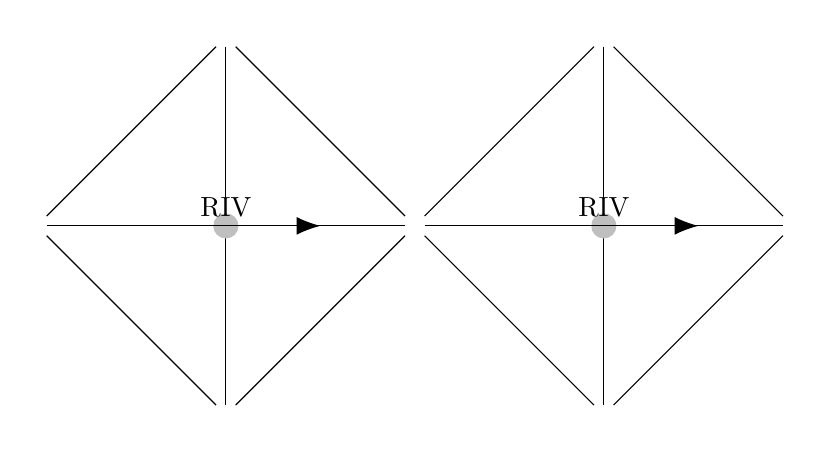
\begin{tikzpicture}[scale=0.8]
    % Define the nodes
    \node (A) at (-3,0) {};
    \node (B) at (3,0) {};
    \node (C) at (0,3) {};
    \node (D) at (0,-3) {};
    
    % Draw the lines
    \draw (A) -- (B);
    \draw (A) -- (C);
    \draw (A) -- (D);
    \draw (B) -- (C);
    \draw (B) -- (D);
    \draw (C) -- (D);
    
    % Highlight the intersection point
    \fill[gray!50] (0,0) circle (0.2);
    
    % Draw the arrow indicating RIV
    \draw[-{Latex[length=3mm]}] (-1.5,0) -- node[midway,above,sloped] {RIV} (1.5,0);

    % Repeat the same for the second part of the diagram
    \begin{scope}[xshift=6cm]
        \node (A) at (-3,0) {};
        \node (B) at (3,0) {};
        \node (C) at (0,3) {};
        \node (D) at (0,-3) {};
        
        \draw (A) -- (B);
        \draw (A) -- (C);
        \draw (A) -- (D);
        \draw (B) -- (C);
        \draw (B) -- (D);
        \draw (C) -- (D);
        
        \fill[gray!50] (0,0) circle (0.2);
        
        \draw[-{Latex[length=3mm]}] (-1.5,0) -- node[midway,above,sloped] {RIV} (1.5,0);
    \end{scope}
\end{tikzpicture}

\end{document}